% FIG:q22-triangle-circle
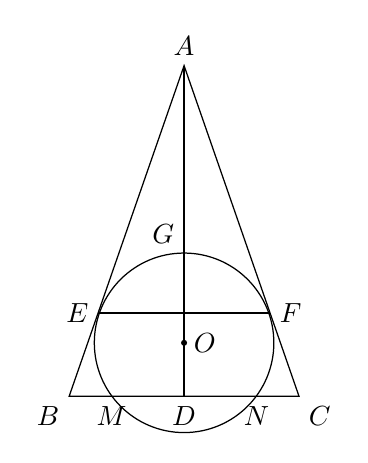
\begin{tikzpicture}[x=1cm,y=1cm,line width=0.45pt]
  \coordinate (A) at (0,4.2);
  \coordinate (B) at (-1.46,0);
  \coordinate (C) at (1.46,0);
  \coordinate (D) at (0,0);
  \coordinate (O) at (0,0.68);
  \coordinate (E) at (-1.09,1.06);
  \coordinate (F) at (1.09,1.06);
  \coordinate (G) at (0,1.82);
  \coordinate (M) at (-0.92,0);
  \coordinate (N) at (0.92,0);
  \draw (A)--(B)--(C)--cycle;
  \draw (0,4.2)--(0,0);
  \draw (O) circle[radius=1.14];
  \draw (E)--(F);
  \fill (O) circle (1.1pt);
  \foreach \p/\pos/\lab in {A/above/A,B/below left/B,C/below right/C,D/below/D,O/right/O,E/left/E,F/right/F,G/above left/G,M/below/M,N/below/N} {
    \node[\pos] at (\p) {$\lab$};
  }
\end{tikzpicture}
